\chapter{Results}
\label{cha:results}

\ldots\todo[inline]{3 pages}

This chapter covers the results from running our implementation on a
fine grid. Random sample points are uniformly selected within a
square of side length \(100 \sqrt{n}\) where \(n\) is the number of
points. This guarantees the same point density for all sample sizes
and seemed to be a sufficient accuracy for real world instances.
All coordinates are integer and transformed back to the unit
square for analysis. For calculations (i.e. within the implementation
itself) we use \verb|double| however.

\section{Technical Details}
All experiments are run on a Intel\textsuperscript{\textregistered}~%
Core\texttrademark~2 Duo CPU E6850 with 2 GB RAM. For everything but
the IP-solving with CPLEX only one core is used. We compile with the
GCC and following options: \verb|-frounding-math -std=c++11 -O3|. The
libraries we compile against are Qt 5.0.0, CGAL 4.0.2, Boost 1.49,
and JSON Spirit 4.06.

\section{Segment Lengths}
\label{sec:results_segments}
\Cref{fig:segment_length,fig:segment_index} show the trend of
the shortest non-separable segment in comparison with the shortest
segment overall and the shortest segment of the \gls{MELT} solution.
For each data point 100 instances were run--though some of them have
been aborted after 30 minutes (refer to \cref{sec:aborted_instances,%
tab:segment_index,tab:segment_length}).

Even though the specific progression of the shortest non-separable
segment index is not clear from \cref{fig:segment_index}, it can be
assumed that it is sub-linear. From \cref{fig:segment_length}, we can
also see that the shortest segment length significantly drops below
the shortest non-separable segment length---which results in more
segments being in between for a uniform distribution.

\begin{landscape}
\begin{figure}[ht]
  \centering
  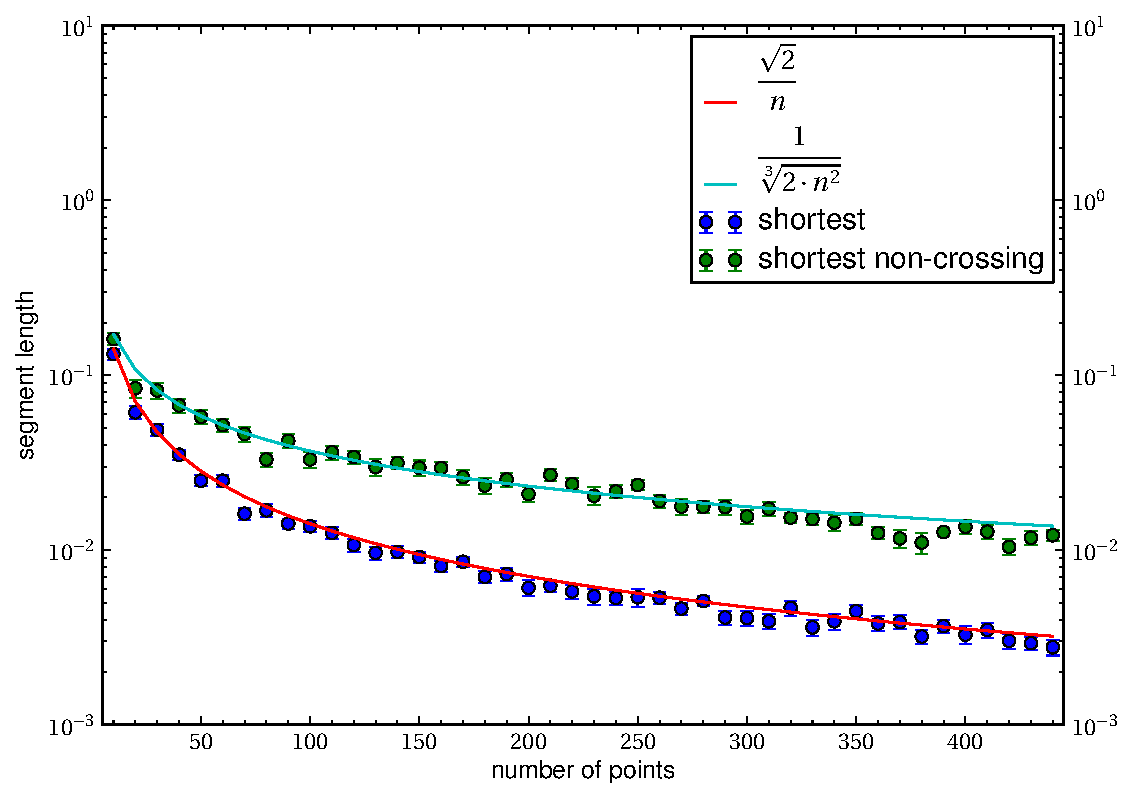
\includegraphics[width=\linewidth,keepaspectratio]{results/segment_length.pdf}
  \caption{\label{fig:segment_length}Comparison of segment lengths}
\end{figure}

\begin{figure}[ht]
  \centering
  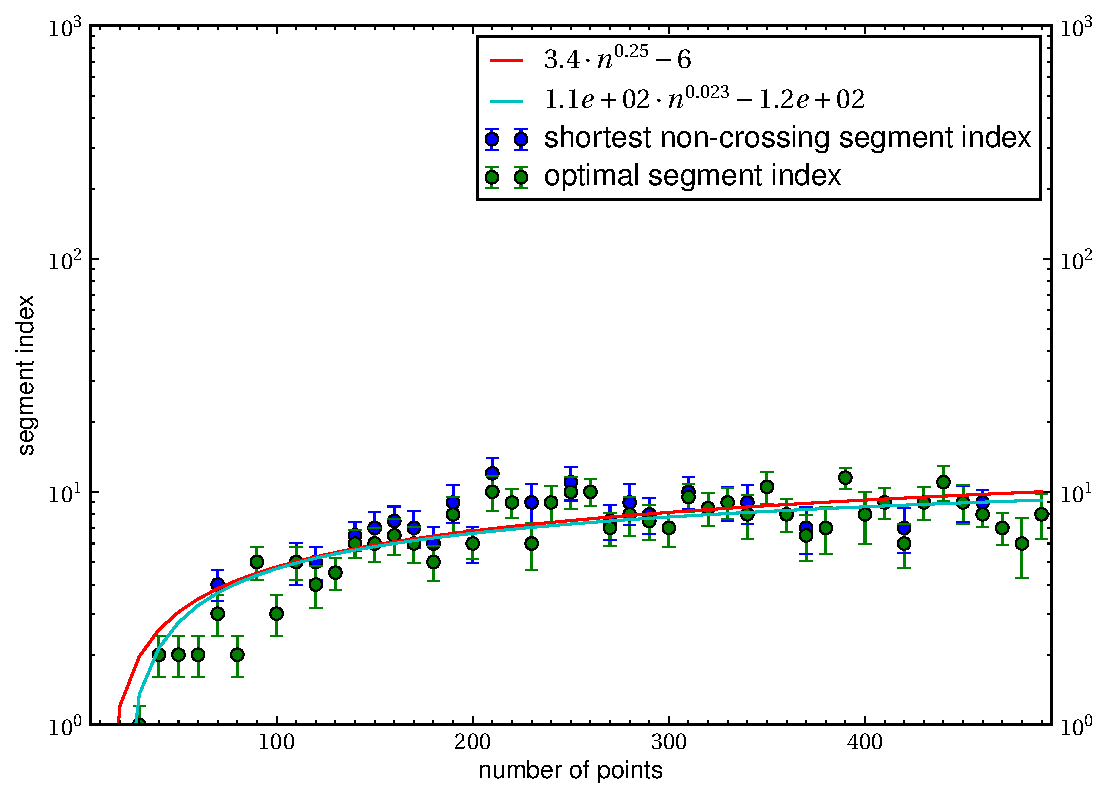
\includegraphics[width=\linewidth,keepaspectratio]{results/segment_index.pdf}
  \caption{\label{fig:segment_index}Comparison of segment indices}
\end{figure}
\end{landscape}

\section{Execution Time}
We made different experimental analyses on the running time of our
implementation. Again we let 100 instances run for each data point.
The resulting times are real time (in contrast to user or system
time)---i.e. execution time of non-related background processes is
not excluded. This decision was made because it is usually impossible
to guarantee that no other (system) tasks are running, so real time
is more meaningful (yet less accurate).

\Cref{fig:time_composition} shows which part of our algorithm takes
what amount of time in comparison to the full execution execution
time. As can 

%---------------------------------------------------------------------##########

\cref{tab:time_composition}

%\newgeometry{margin=1.5cm}
%\begin{landscape}
\begin{figure}[ht]
  \centering
  %\thisfloatpagestyle{empty}
  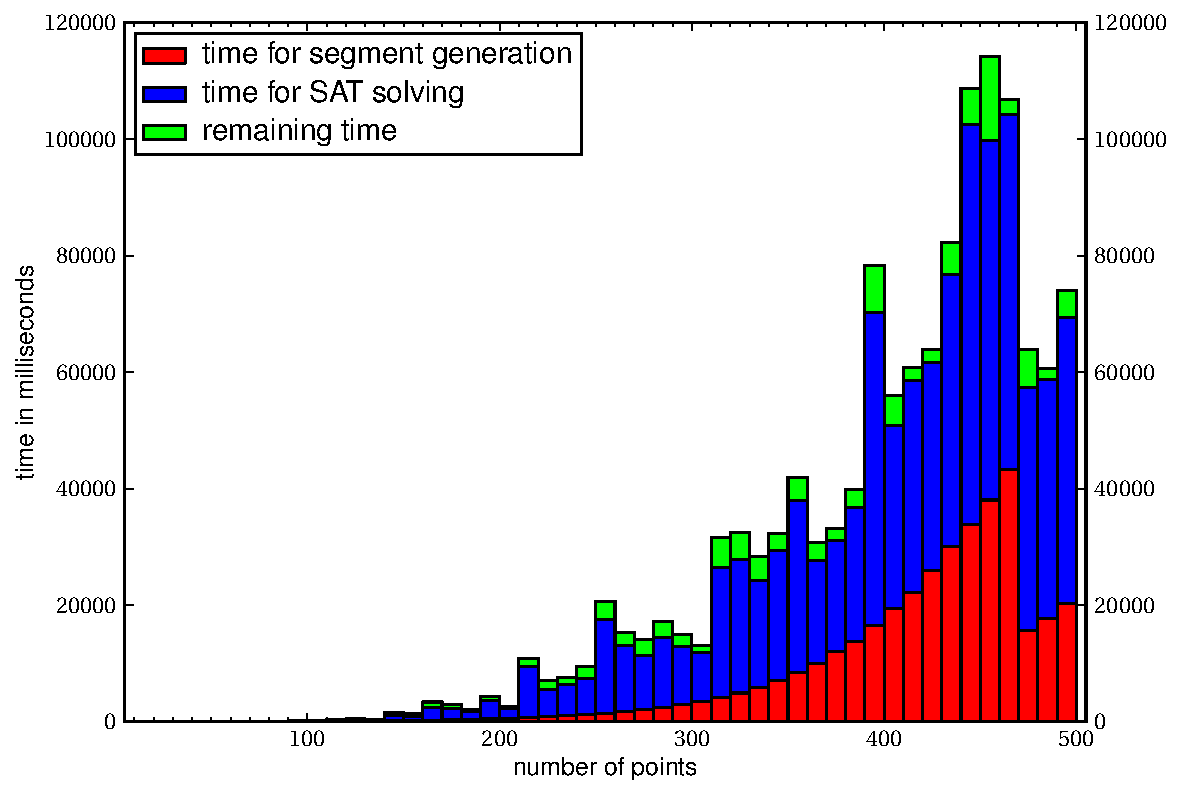
\includegraphics
  [width=\linewidth,height=\textheight,keepaspectratio]
  {results/time_composition.pdf}
  \caption{\label{fig:time_composition}Composition of execution times}
\end{figure}
%\end{landscape}
%\restoregeometry

\begin{figure}[ht]
  \centering
  \begin{subfigure}{\textwidth}
    \centering
    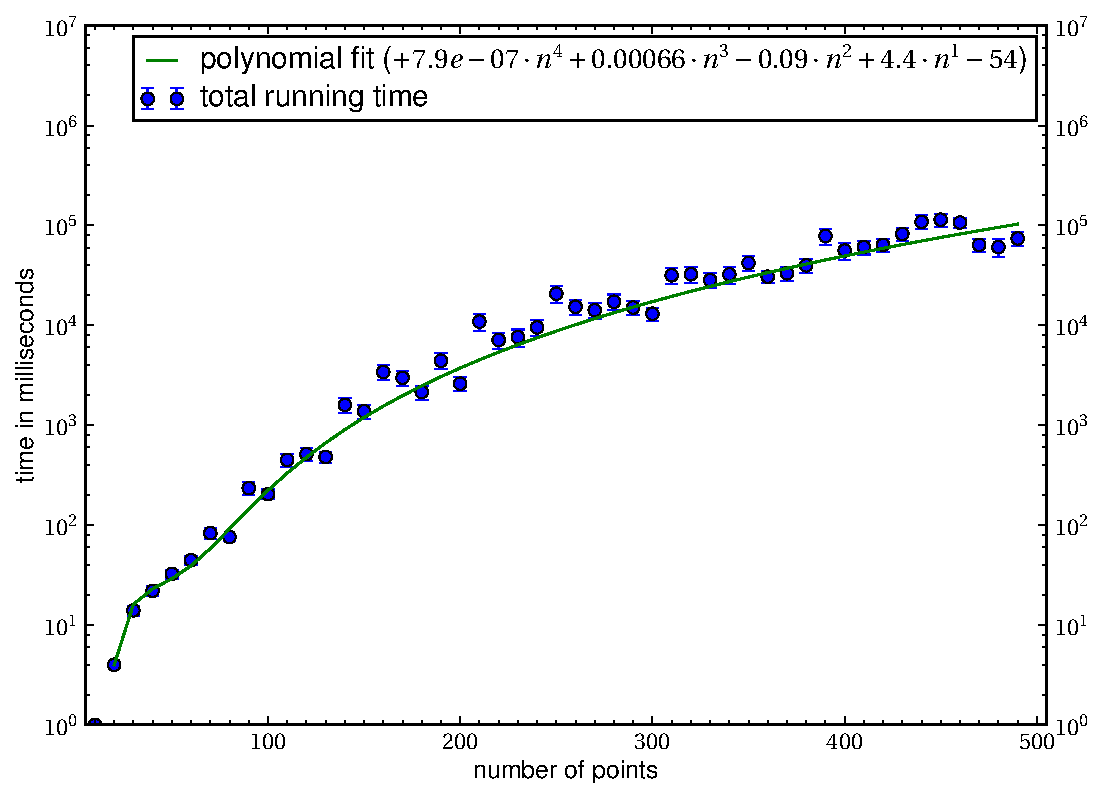
\includegraphics
    [width=\linewidth,height=\textheight,keepaspectratio]
    {results/time_total.pdf}
    \caption{Improved method}
  \end{subfigure}
  
  \begin{subfigure}{\textwidth}
    \centering
    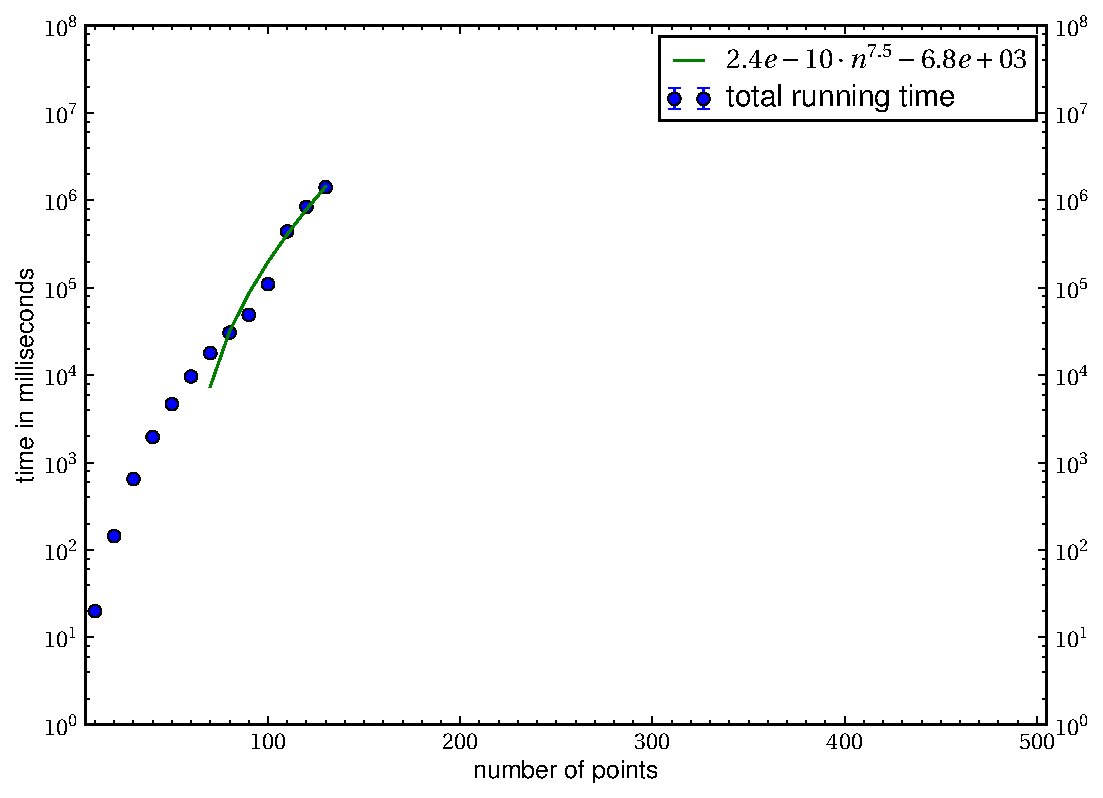
\includegraphics
    [width=\linewidth,height=\textheight,keepaspectratio]
    {results/complete_sat/time_total.pdf}
    \caption{Complete SAT}
  \end{subfigure}
  \caption{\label{fig:time_total}Total execution time}
\end{figure}

\begin{figure}[ht]
  \centering
  \begin{subfigure}{\textwidth}
    \centering
    \includegraphics%
    [width=\linewidth,height=\textheight,keepaspectratio]
    {results/time_hist_0070.pdf}
    \caption{\label{fig:times_70}70 points}
  \end{subfigure}
  
  \begin{subfigure}{\textwidth}
    \centering
    \includegraphics%
    [width=\linewidth,height=\textheight,keepaspectratio]
    {results/time_hist_0080.pdf}
    \caption{\label{fig:times_80}80 points}
  \end{subfigure}
  \caption{Histogram of execution times}
\end{figure}

\section{Aborted instances}
\label{sec:aborted_instances}

%\newgeometry{margin=1.5cm}
%\begin{landscape}
\begin{figure}[ht]
  \centering
  \begin{subfigure}{\textwidth}
    \centering
    \includegraphics%
    [width=\linewidth,height=0.4\textheight,keepaspectratio]%
    {results/complete_sat/time_hist.pdf}
    \caption{Complete SAT}
  \end{subfigure}
  
  \begin{subfigure}{\textwidth}
    \centering
    \includegraphics%
    [width=\linewidth,height=0.4\textheight,keepaspectratio]%
    {results/time_hist.pdf}
    \caption{Improved method}
  \end{subfigure}
  \caption{Instances with running time < 23:20min}
\end{figure}
%\end{landscape}
%\restoregeometry
